\section{\tl{MCA vs MCA - DCCA}}
\en{Moving on from the classification of the raw data versus the DCCA transformed data, we explore the effect that MCA has, and introduce the results of the classification. In this part, we present the classification results, (a) of the data after the genetic view has been transformed through MCA, and (b) of the DCCA transformed data after the genetic view has been transformed through MCA.}

\subsection{\en{Without scaling or balancing:}}
\en{
\begin{figure}[H]
    \centering
    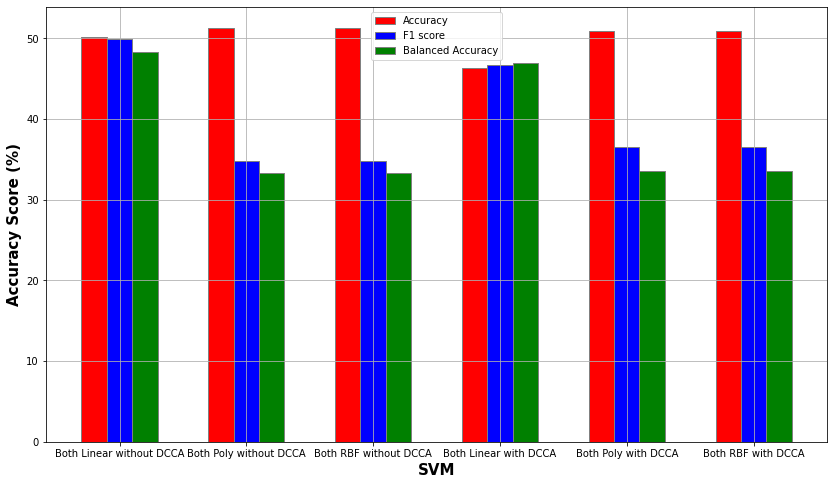
\includegraphics[width=\textwidth]{figures/Results/MCA/MCA_Both_out.png}
    \caption[\en{Classification metric scores using Both views on MCA vs MCA-DCCA data}]{\en{Classification metric scores using Both views (Imaging and Genetic), on the SVM kernels (Linear, Polynomial, RBF), using raw imaging and MCA transformed genetic data (3 left bar groups) vs using DCCA transformed raw imaging and MCA transformed genetic data (3 right bar groups)}}
\end{figure}

\begin{figure}[H]
    \centering
    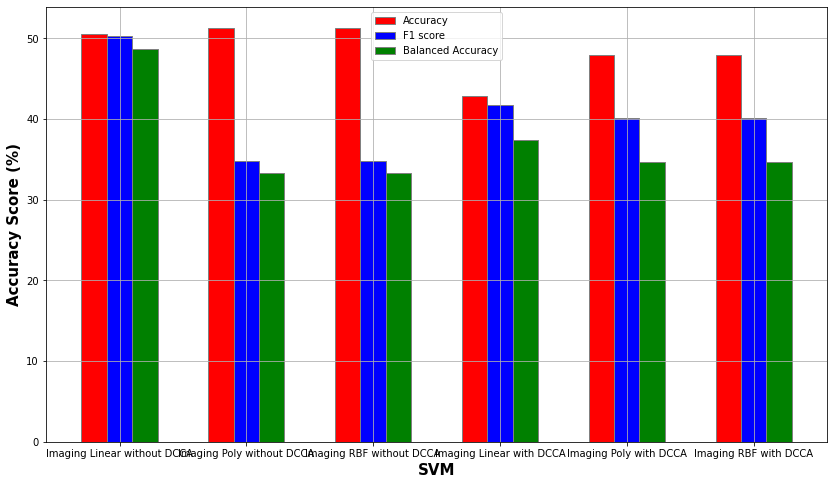
\includegraphics[width=\textwidth]{figures/Results/MCA/MCA_Ima_out.png}
    \caption[\en{Classification metric scores using Imaging view on MCA vs MCA-DCCA data}]{\en{Classification metric scores using only the Imaging view, on the SVM kernels (Linear, Polynomial, RBF), using raw imaging data (3 left bar groups) vs using the DCCA transformed imaging data, trained on raw imaging data and MCA transformed genetic data (3 right bar groups).}}
\end{figure}

\begin{figure}[H]
    \centering
    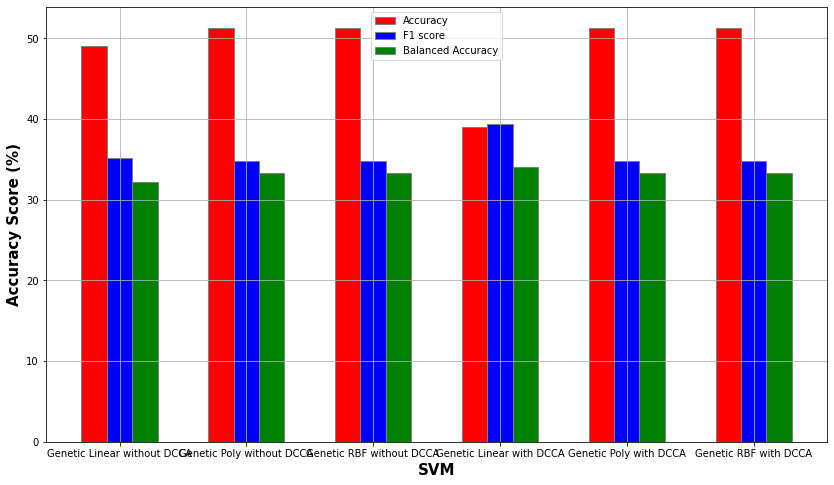
\includegraphics[width=\textwidth]{figures/Results/MCA/MCA_Gen_out.png}
    \caption[\en{Classification metric scores using Genetic view on MCA vs MCA-DCCA data}]{\en{Classification metric scores using only the genetic view, on the SVM kernels (Linear, Polynomial, RBF), using MCA transformed genetic data (3 left bar groups) vs using the DCCA transformed genetic data, trained on raw imaging data and MCA transformed genetic data (3 right bar groups).}}
\end{figure}

% \begin{figure}[H]
%     \centering
%     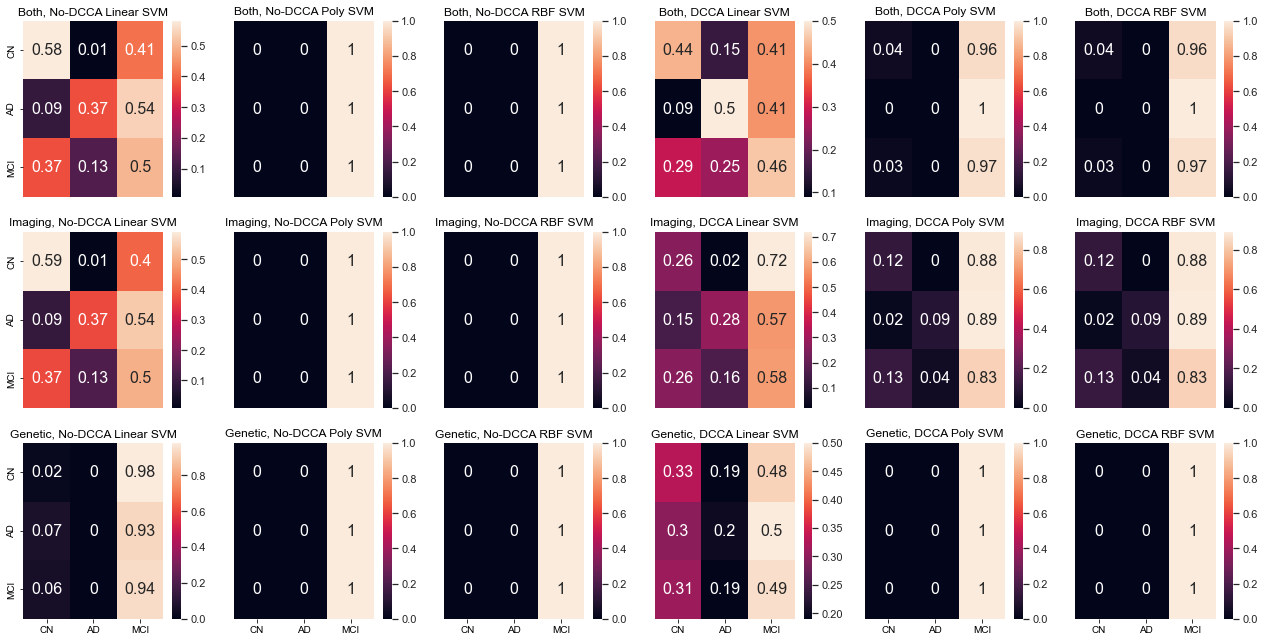
\includegraphics[width=\textwidth]{figures/Results/MCA/MCA_CM_out.png}
%     \caption[\en{Confusion Matrices of MCA vs MCA-DCCA data}]{\en{The Confusion Matrices for each class, per model, using both views (top row), only the imaging view (middle row), and only the genetic view (bottom row). The three left columns represent the CM of the raw imaging and MCA transformed genetic data classification, while the three right columns represent the CM of the DCCA transformed data classification.}}
% \end{figure}

\begin{figure}[H]
    \centering
    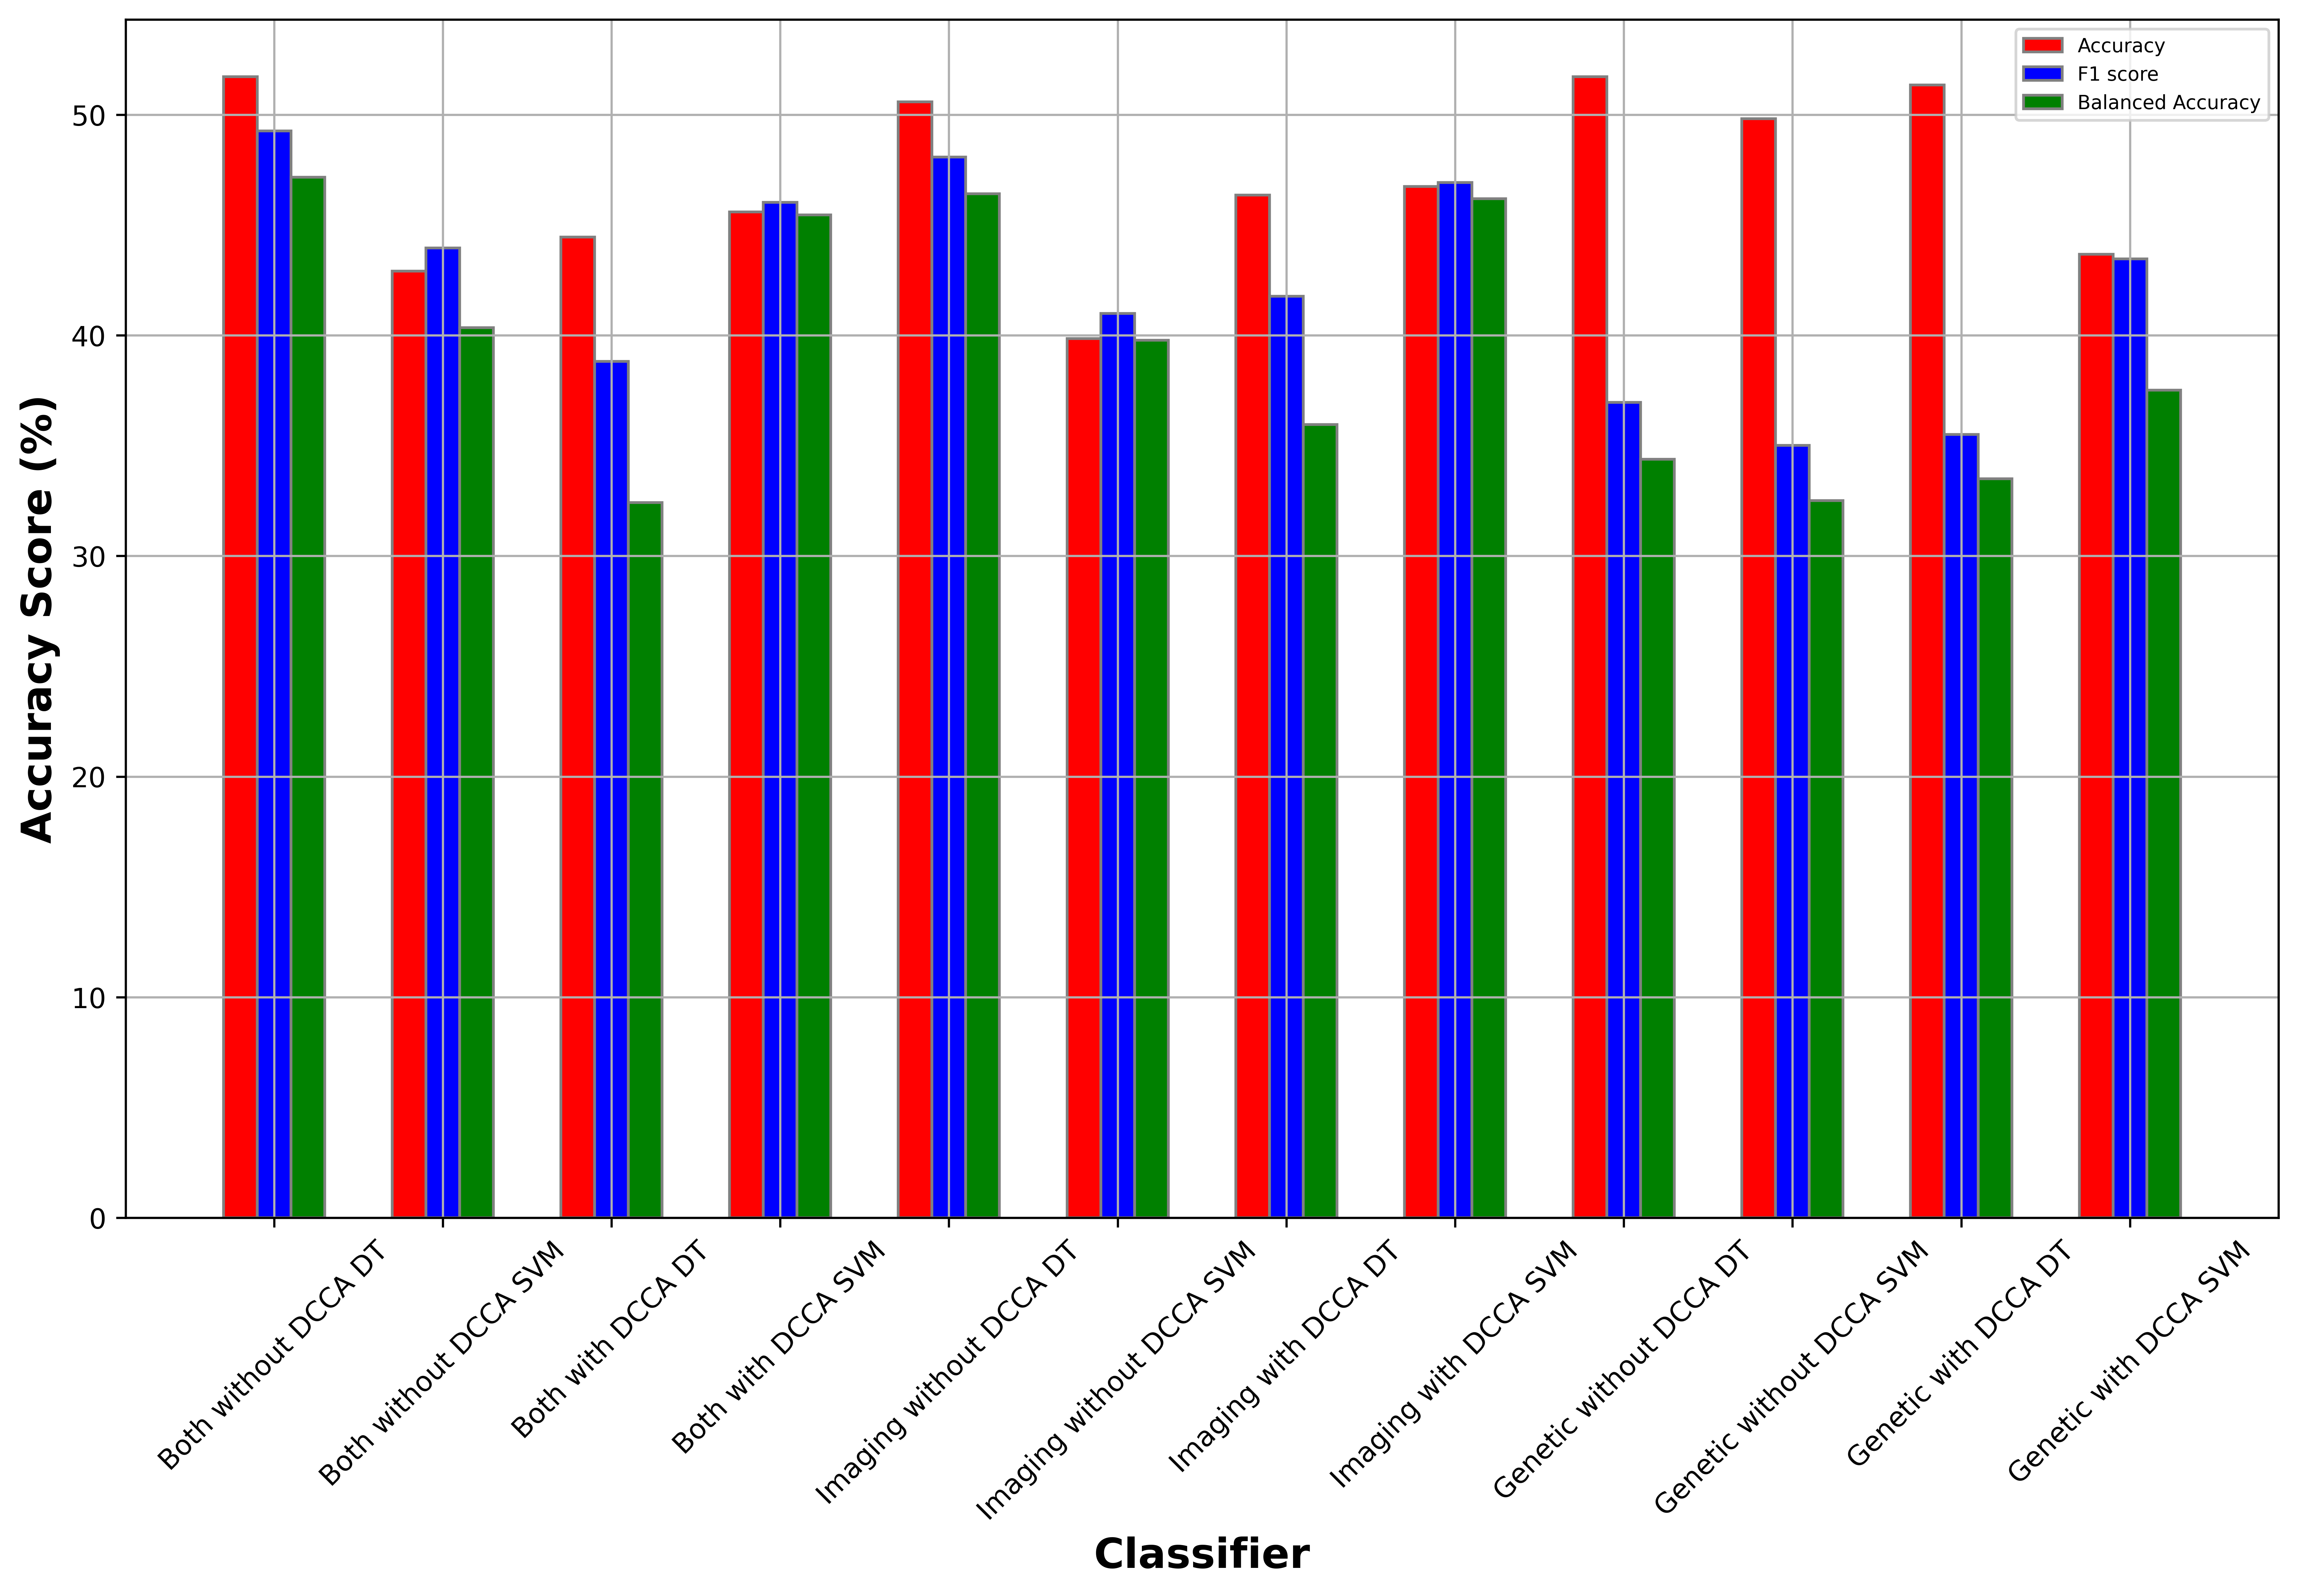
\includegraphics[width=\textwidth]{figures/Results/MCA/Bagging_MCA_out.png}
    \caption[\en{MCA Bagging Classification metrics}]{\en{Classification metric using Bagging on the MCA transformed imaging and genetic data.}}
\end{figure}

% \begin{figure}[H]
%     \centering
%     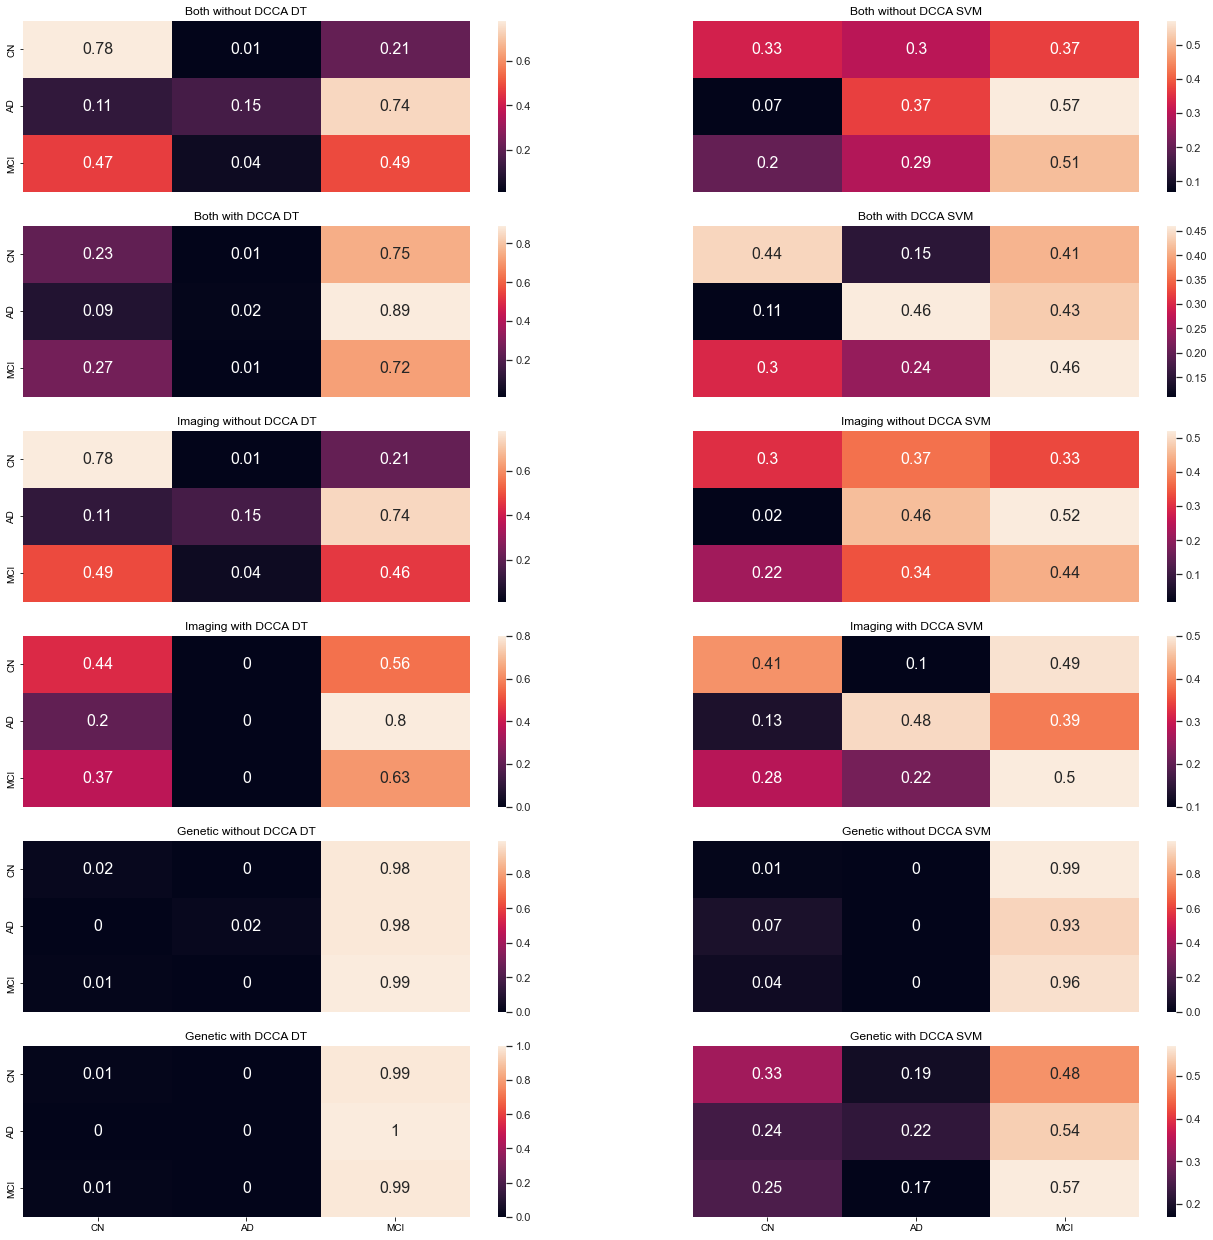
\includegraphics[width=\textwidth]{figures/Results/MCA/Bagging_MCA_CM_out.png}
%     \caption[\en{MCA Bagging Confusion Matrices}]{\en{The Confusion Matrices for each class, with Bagging, for the MCA transformed imaging and genetic data.}}
% \end{figure}

\begin{figure}[H]
    \centering
    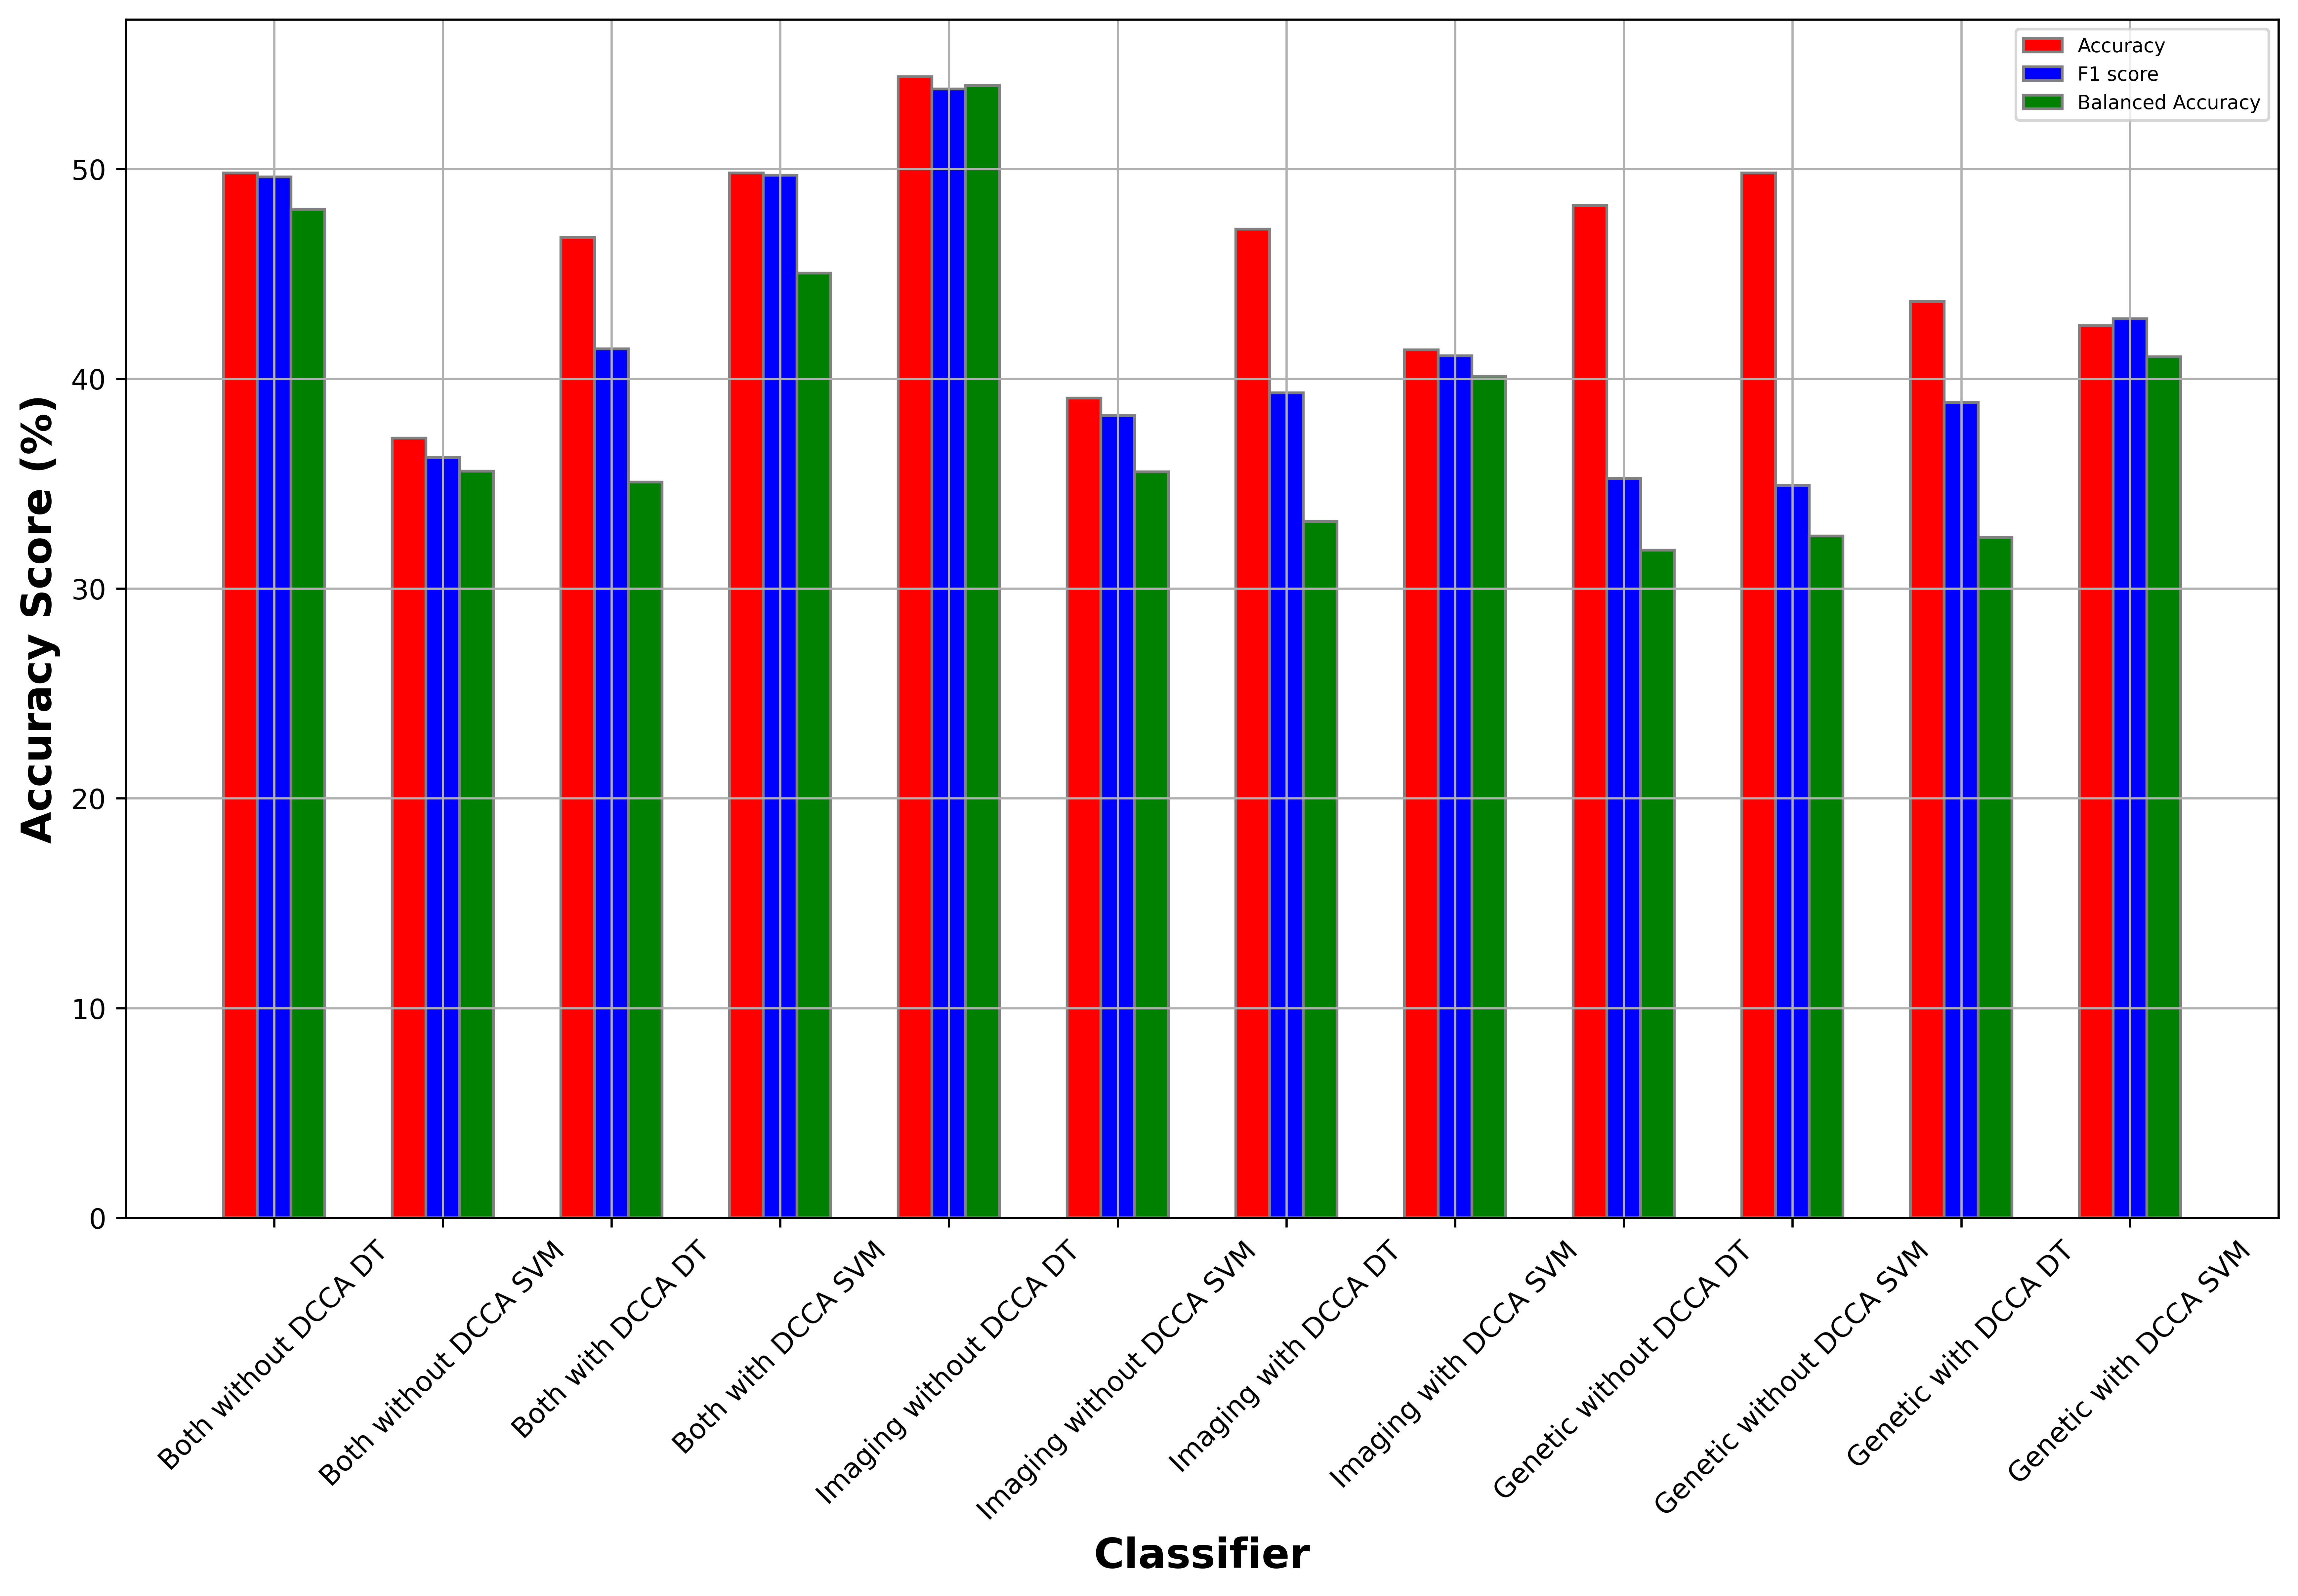
\includegraphics[width=\textwidth]{figures/Results/MCA/AdaBoost_MCA_out.png}
    \caption[\en{MCA AdaBoost Classification metrics}]{\en{Classification metric using AdaBoost on the MCA transformed imaging and genetic data.}}
\end{figure}

% \begin{figure}[H]
%     \centering
%     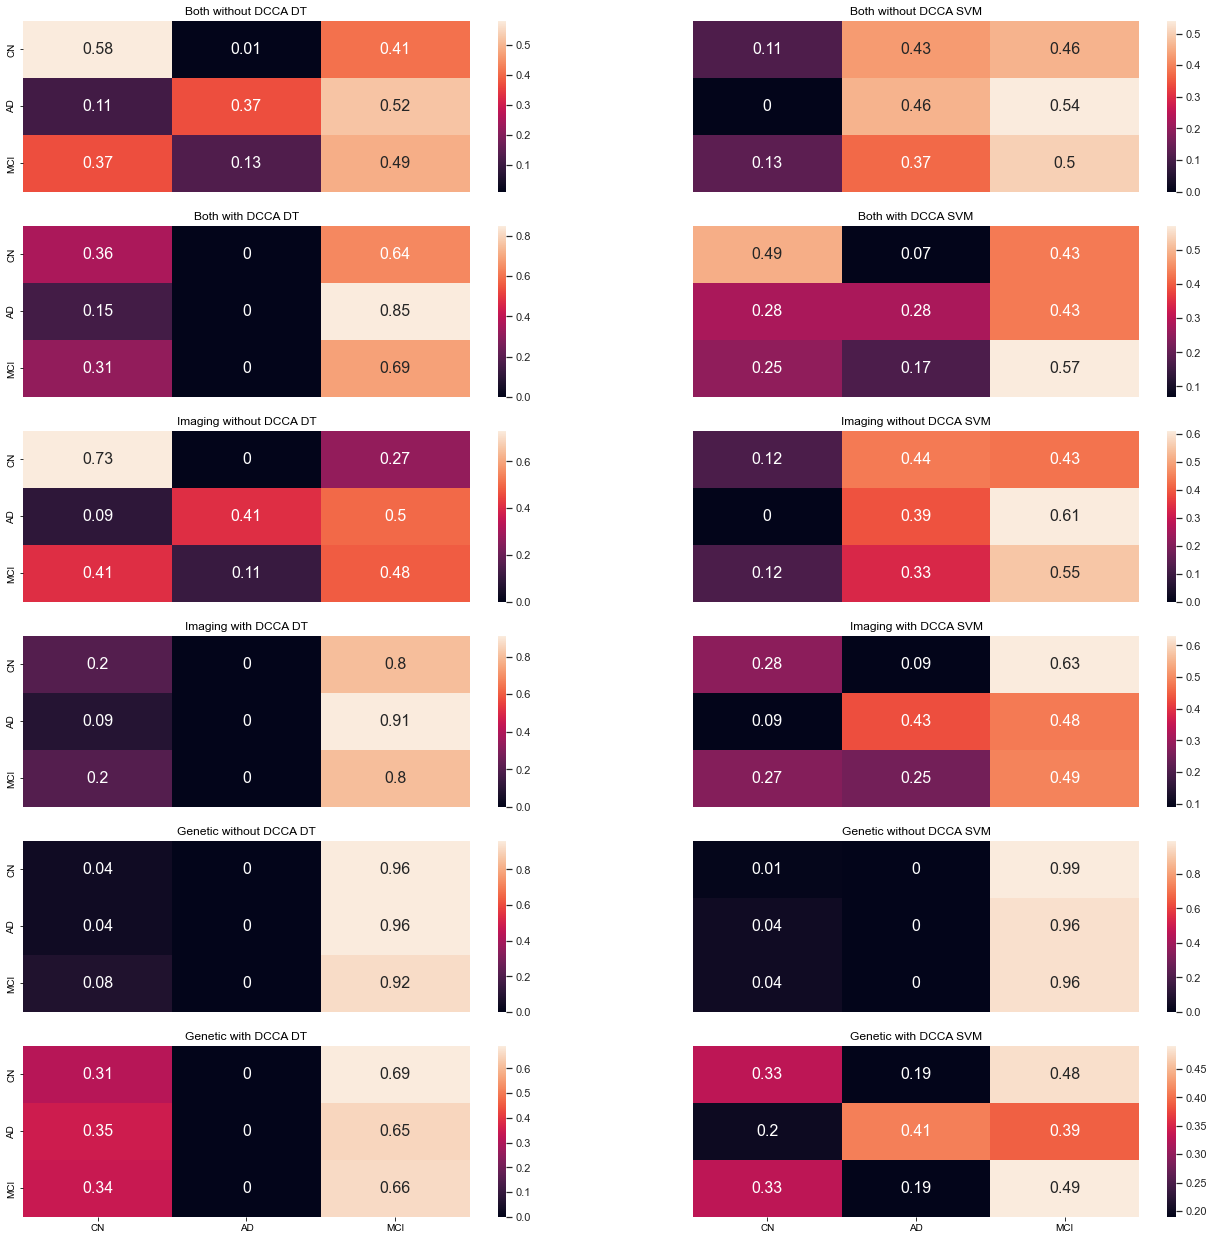
\includegraphics[width=\textwidth]{figures/Results/MCA/AdaBoost_MCA_CM_out.png}
%     \caption[\en{MCA AdaBoost Confusion Matrices}]{\en{The Confusion Matrices for each class, with AdaBoost, for the MCA transformed imaging and genetic data.}}
% \end{figure}

}
\subsection{\en{With scaling and balancing:}}
\en{
\begin{figure}[H]
    \centering
    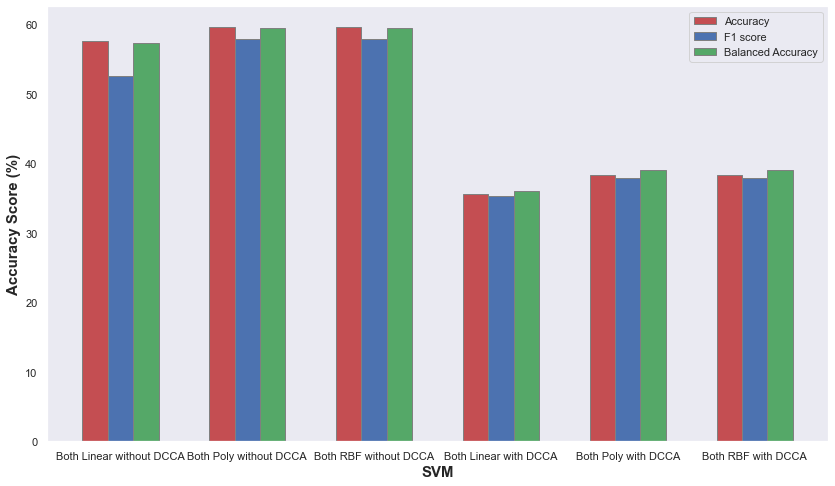
\includegraphics[width=\textwidth]{figures/Results/MCA/MCA_Both_with.png}
    \caption[\en{Classification metric scores using Both views on MCA vs MCA-DCCA data with scaling and balancing}]{\en{Classification metric scores using Both views (Imaging and Genetic), on the SVM kernels (Linear, Polynomial, RBF), using raw imaging and MCA transformed genetic data (3 left bar groups) vs using DCCA transformed raw imaging and MCA transformed genetic data (3 right bar groups)}}
\end{figure}

\begin{figure}[H]
    \centering
    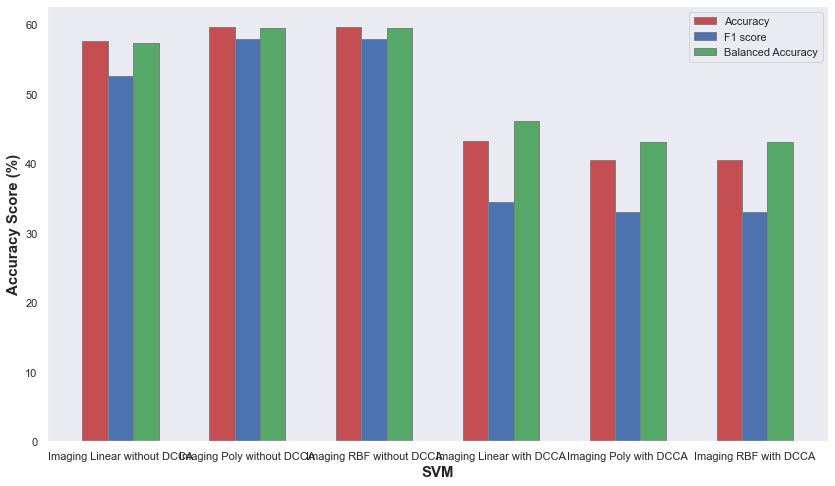
\includegraphics[width=\textwidth]{figures/Results/MCA/MCA_Ima_with.png}
    \caption[\en{Classification metric scores using Imaging view on MCA vs MCA-DCCA data with scaling and balancing}]{\en{Classification metric scores using only the Imaging view, on the SVM kernels (Linear, Polynomial, RBF), using raw imaging data (3 left bar groups) vs using the DCCA transformed imaging data, trained on raw imaging data and MCA transformed genetic data (3 right bar groups).}}
\end{figure}

\begin{figure}[H]
    \centering
    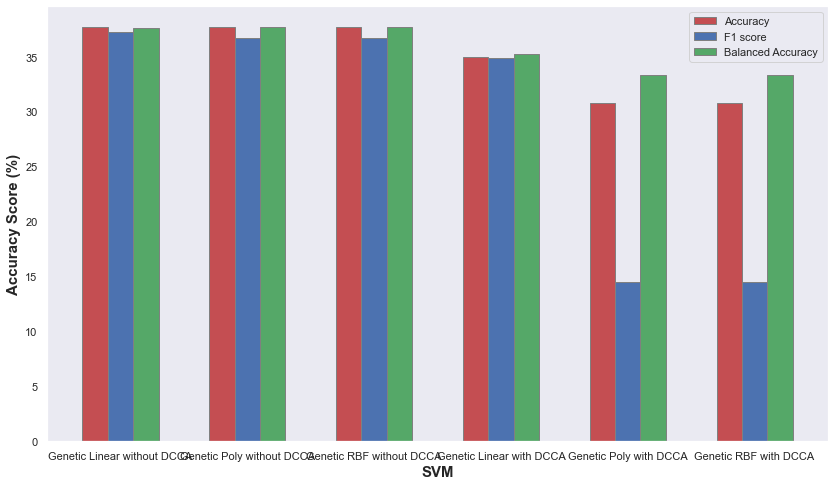
\includegraphics[width=\textwidth]{figures/Results/MCA/MCA_Gen_with.png}
    \caption[\en{Classification metric scores using Genetic view on MCA vs MCA-DCCA data with scaling and balancing}]{\en{Classification metric scores using only the genetic view, on the SVM kernels (Linear, Polynomial, RBF), using MCA transformed genetic data (3 left bar groups) vs using the DCCA transformed genetic data, trained on raw imaging data and MCA transformed genetic data (3 right bar groups).}}
\end{figure}

The confusion matrices of the MCA and MCA - DCCA models are shown, because they performed exceptionally good:
\begin{figure}[H]
    \centering
    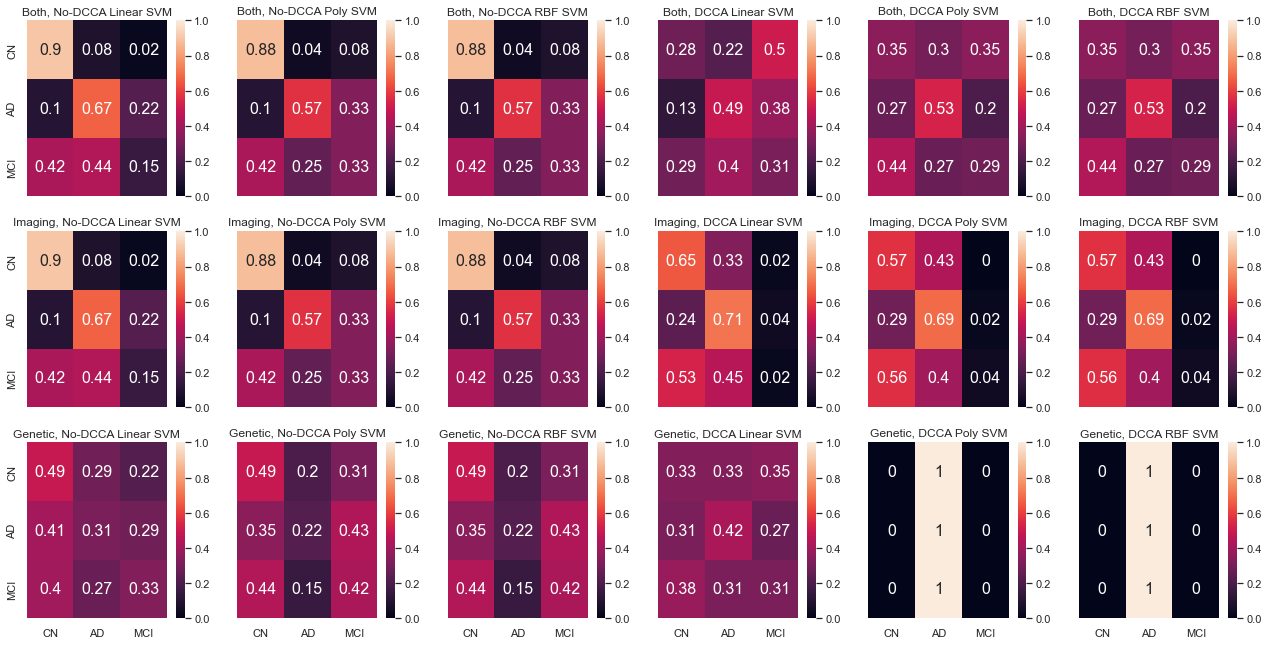
\includegraphics[width=\textwidth]{figures/Results/MCA/MCA_CM_with.png}
    \caption[\en{Confusion Matrices of MCA vs MCA-DCCA data with scaling and balancing}]{\en{The Confusion Matrices for each class, per model, using both views (top row), only the imaging view (middle row), and only the genetic view (bottom row). The three left columns represent the CM of the raw imaging and MCA transformed genetic data classification, while the three right columns represent the CM of the DCCA transformed data classification.}}
    \label{fig:Confusion Matrices of MCA vs MCA-DCCA data with scaling and balancing}
\end{figure}

\begin{figure}[H]
    \centering
    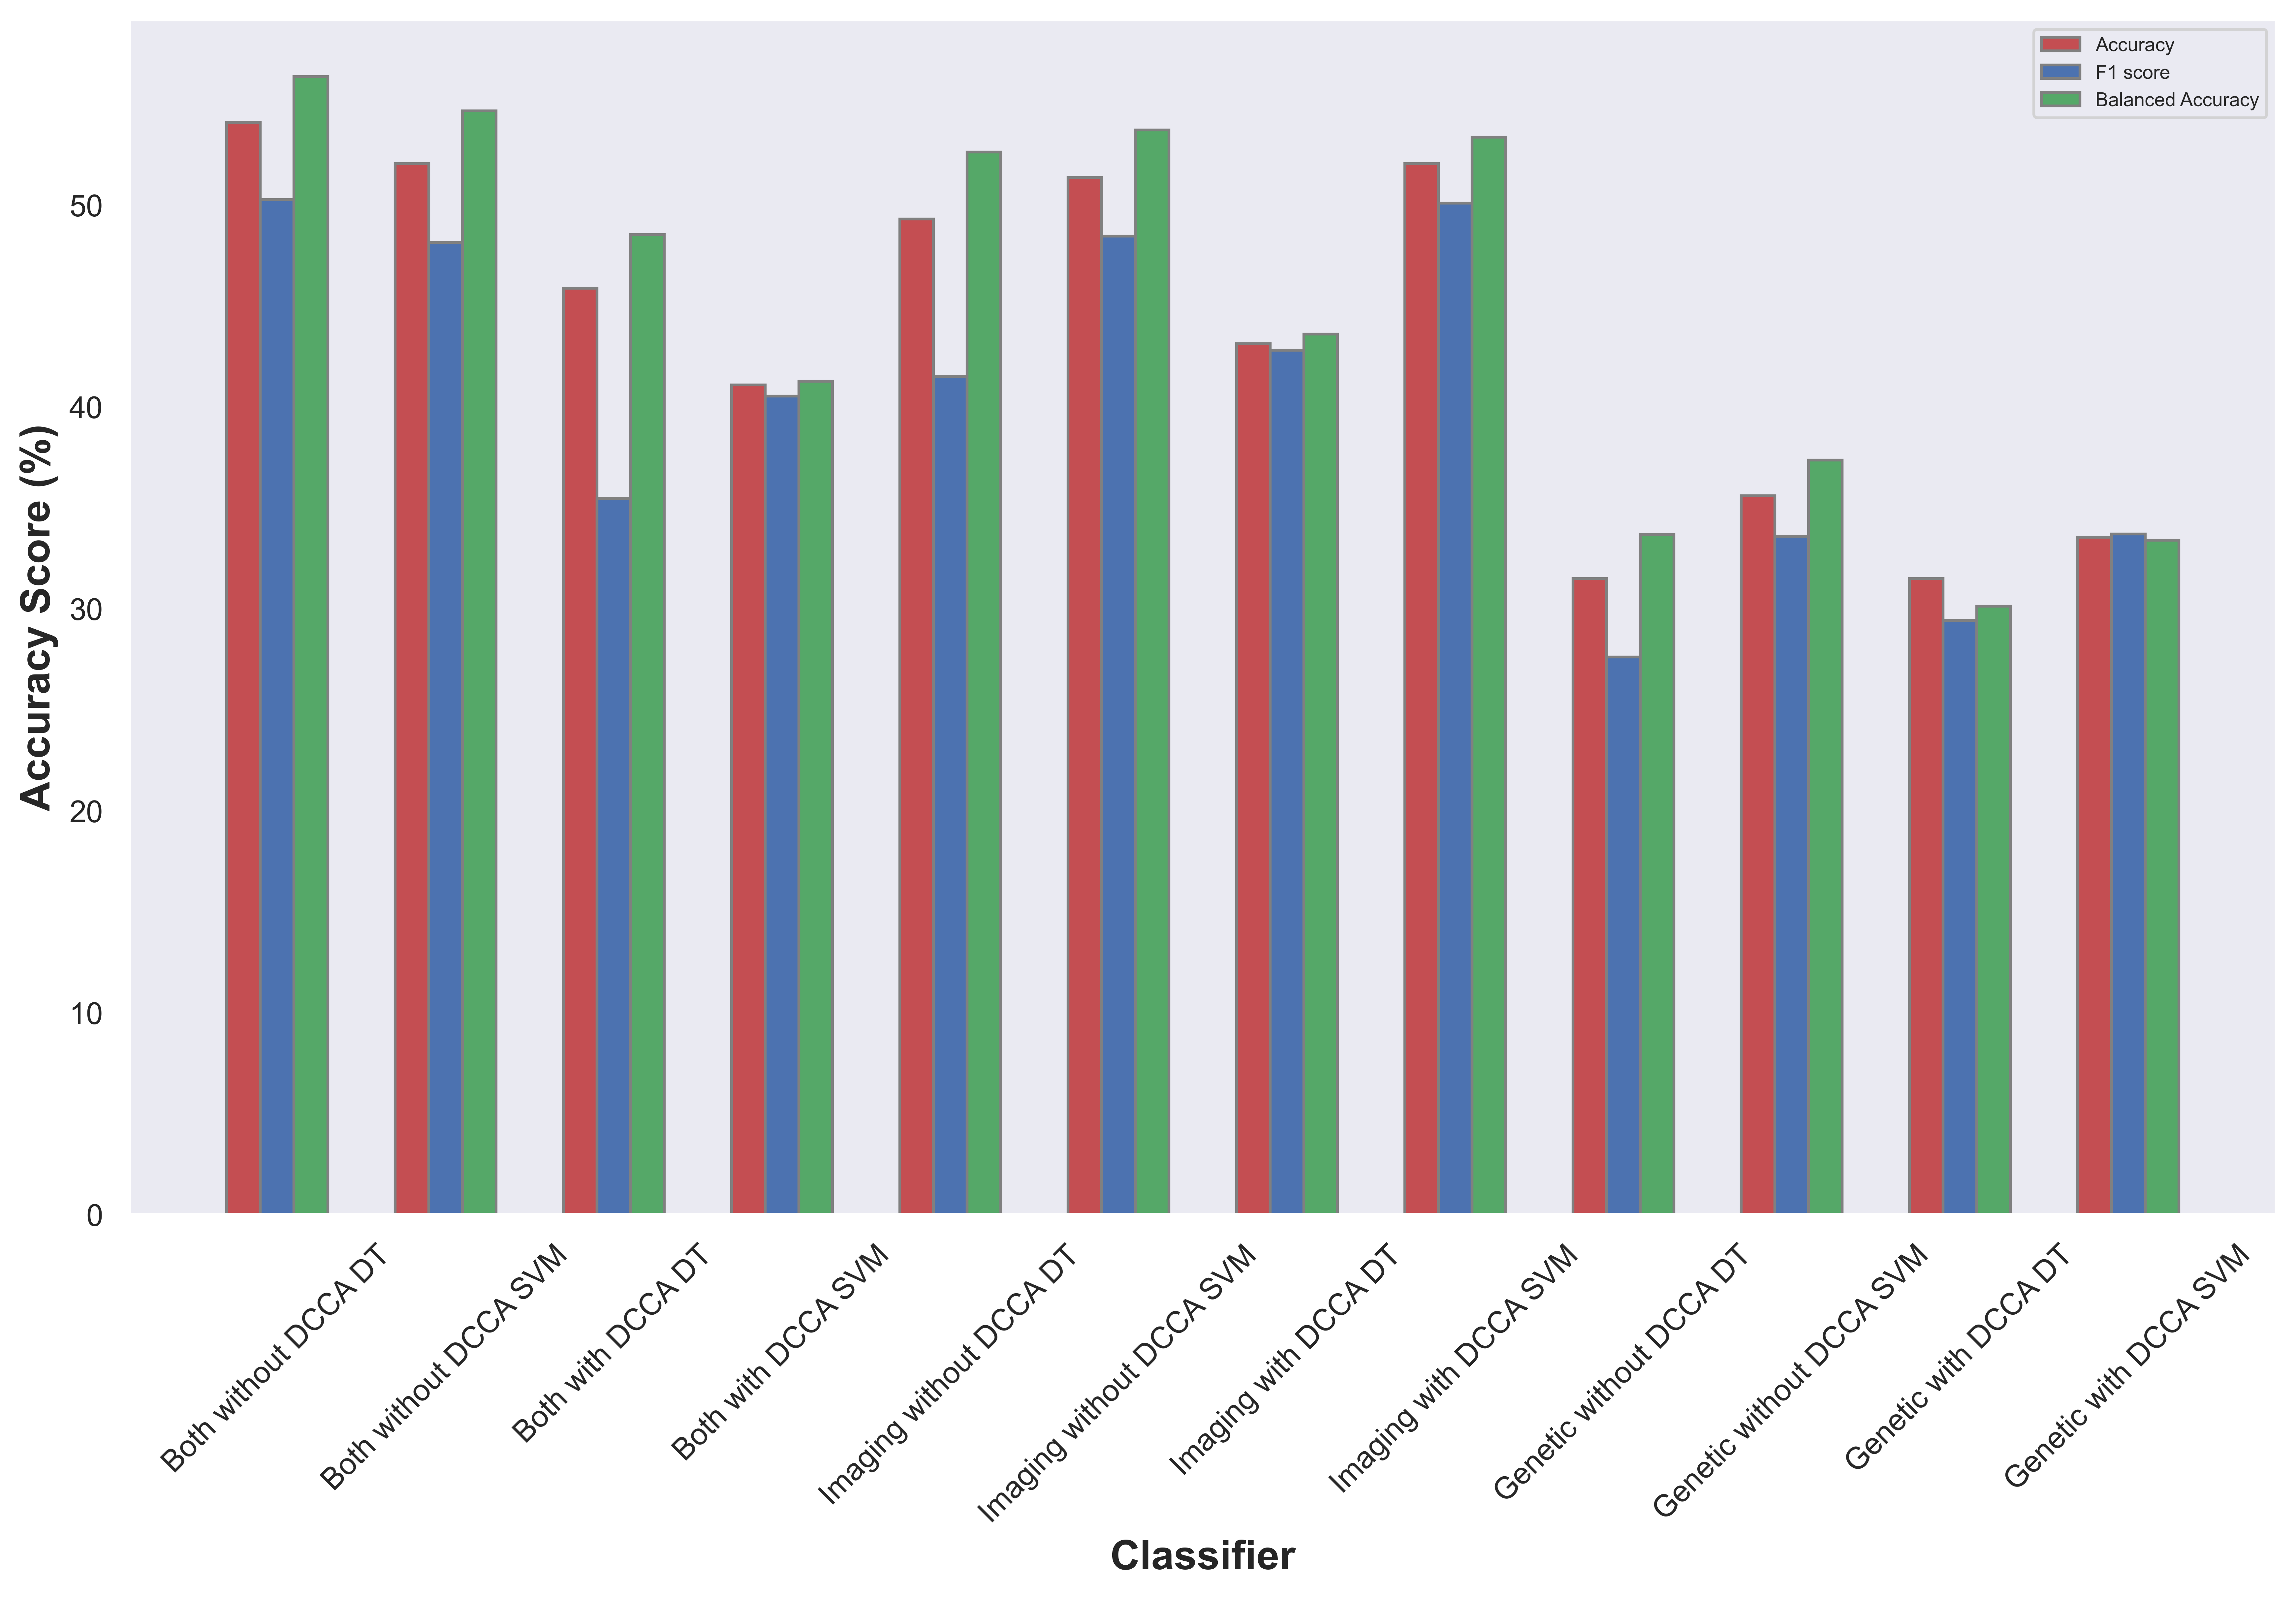
\includegraphics[width=\textwidth]{figures/Results/MCA/Bagging_MCA_with.png}
    \caption[\en{MCA Bagging Classification metrics with scaling and balancing}]{\en{Classification metric using Bagging on the MCA transformed imaging and genetic data.}}
\end{figure}

% \begin{figure}[H]
%     \centering
%     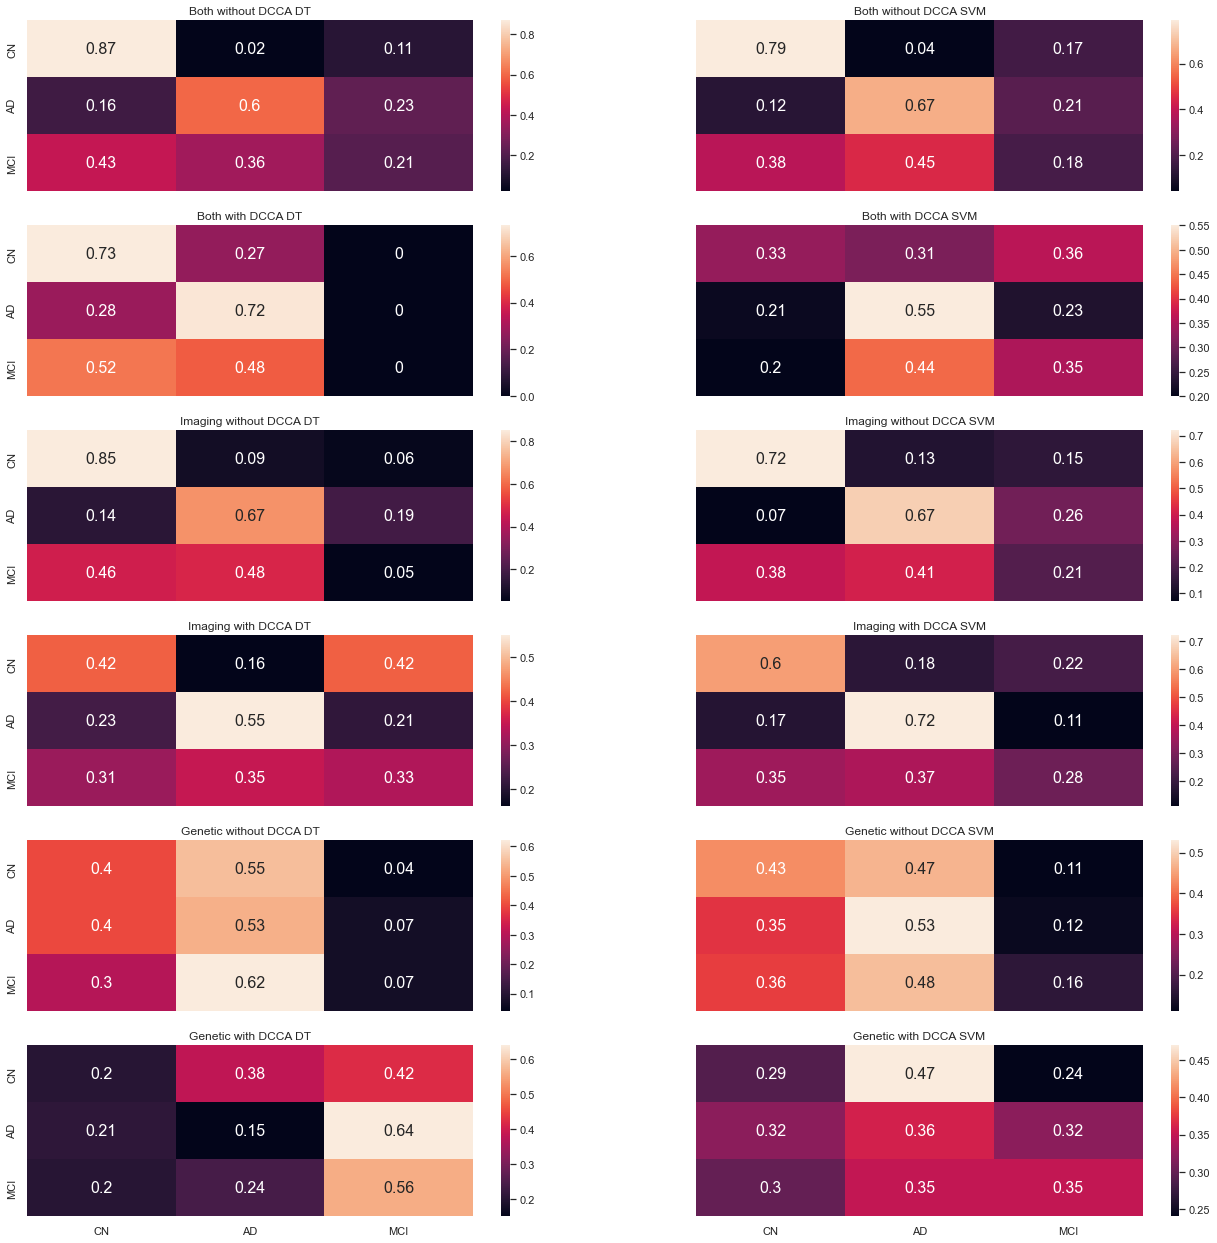
\includegraphics[width=\textwidth]{figures/Results/MCA/Bagging_MCA_CM_with.png}
%     \caption[\en{MCA Bagging Confusion Matrices with scaling and balancing}]{\en{The Confusion Matrices for each class, with Bagging, for the MCA transformed imaging and genetic data.}}
% \end{figure}

\begin{figure}[H]
    \centering
    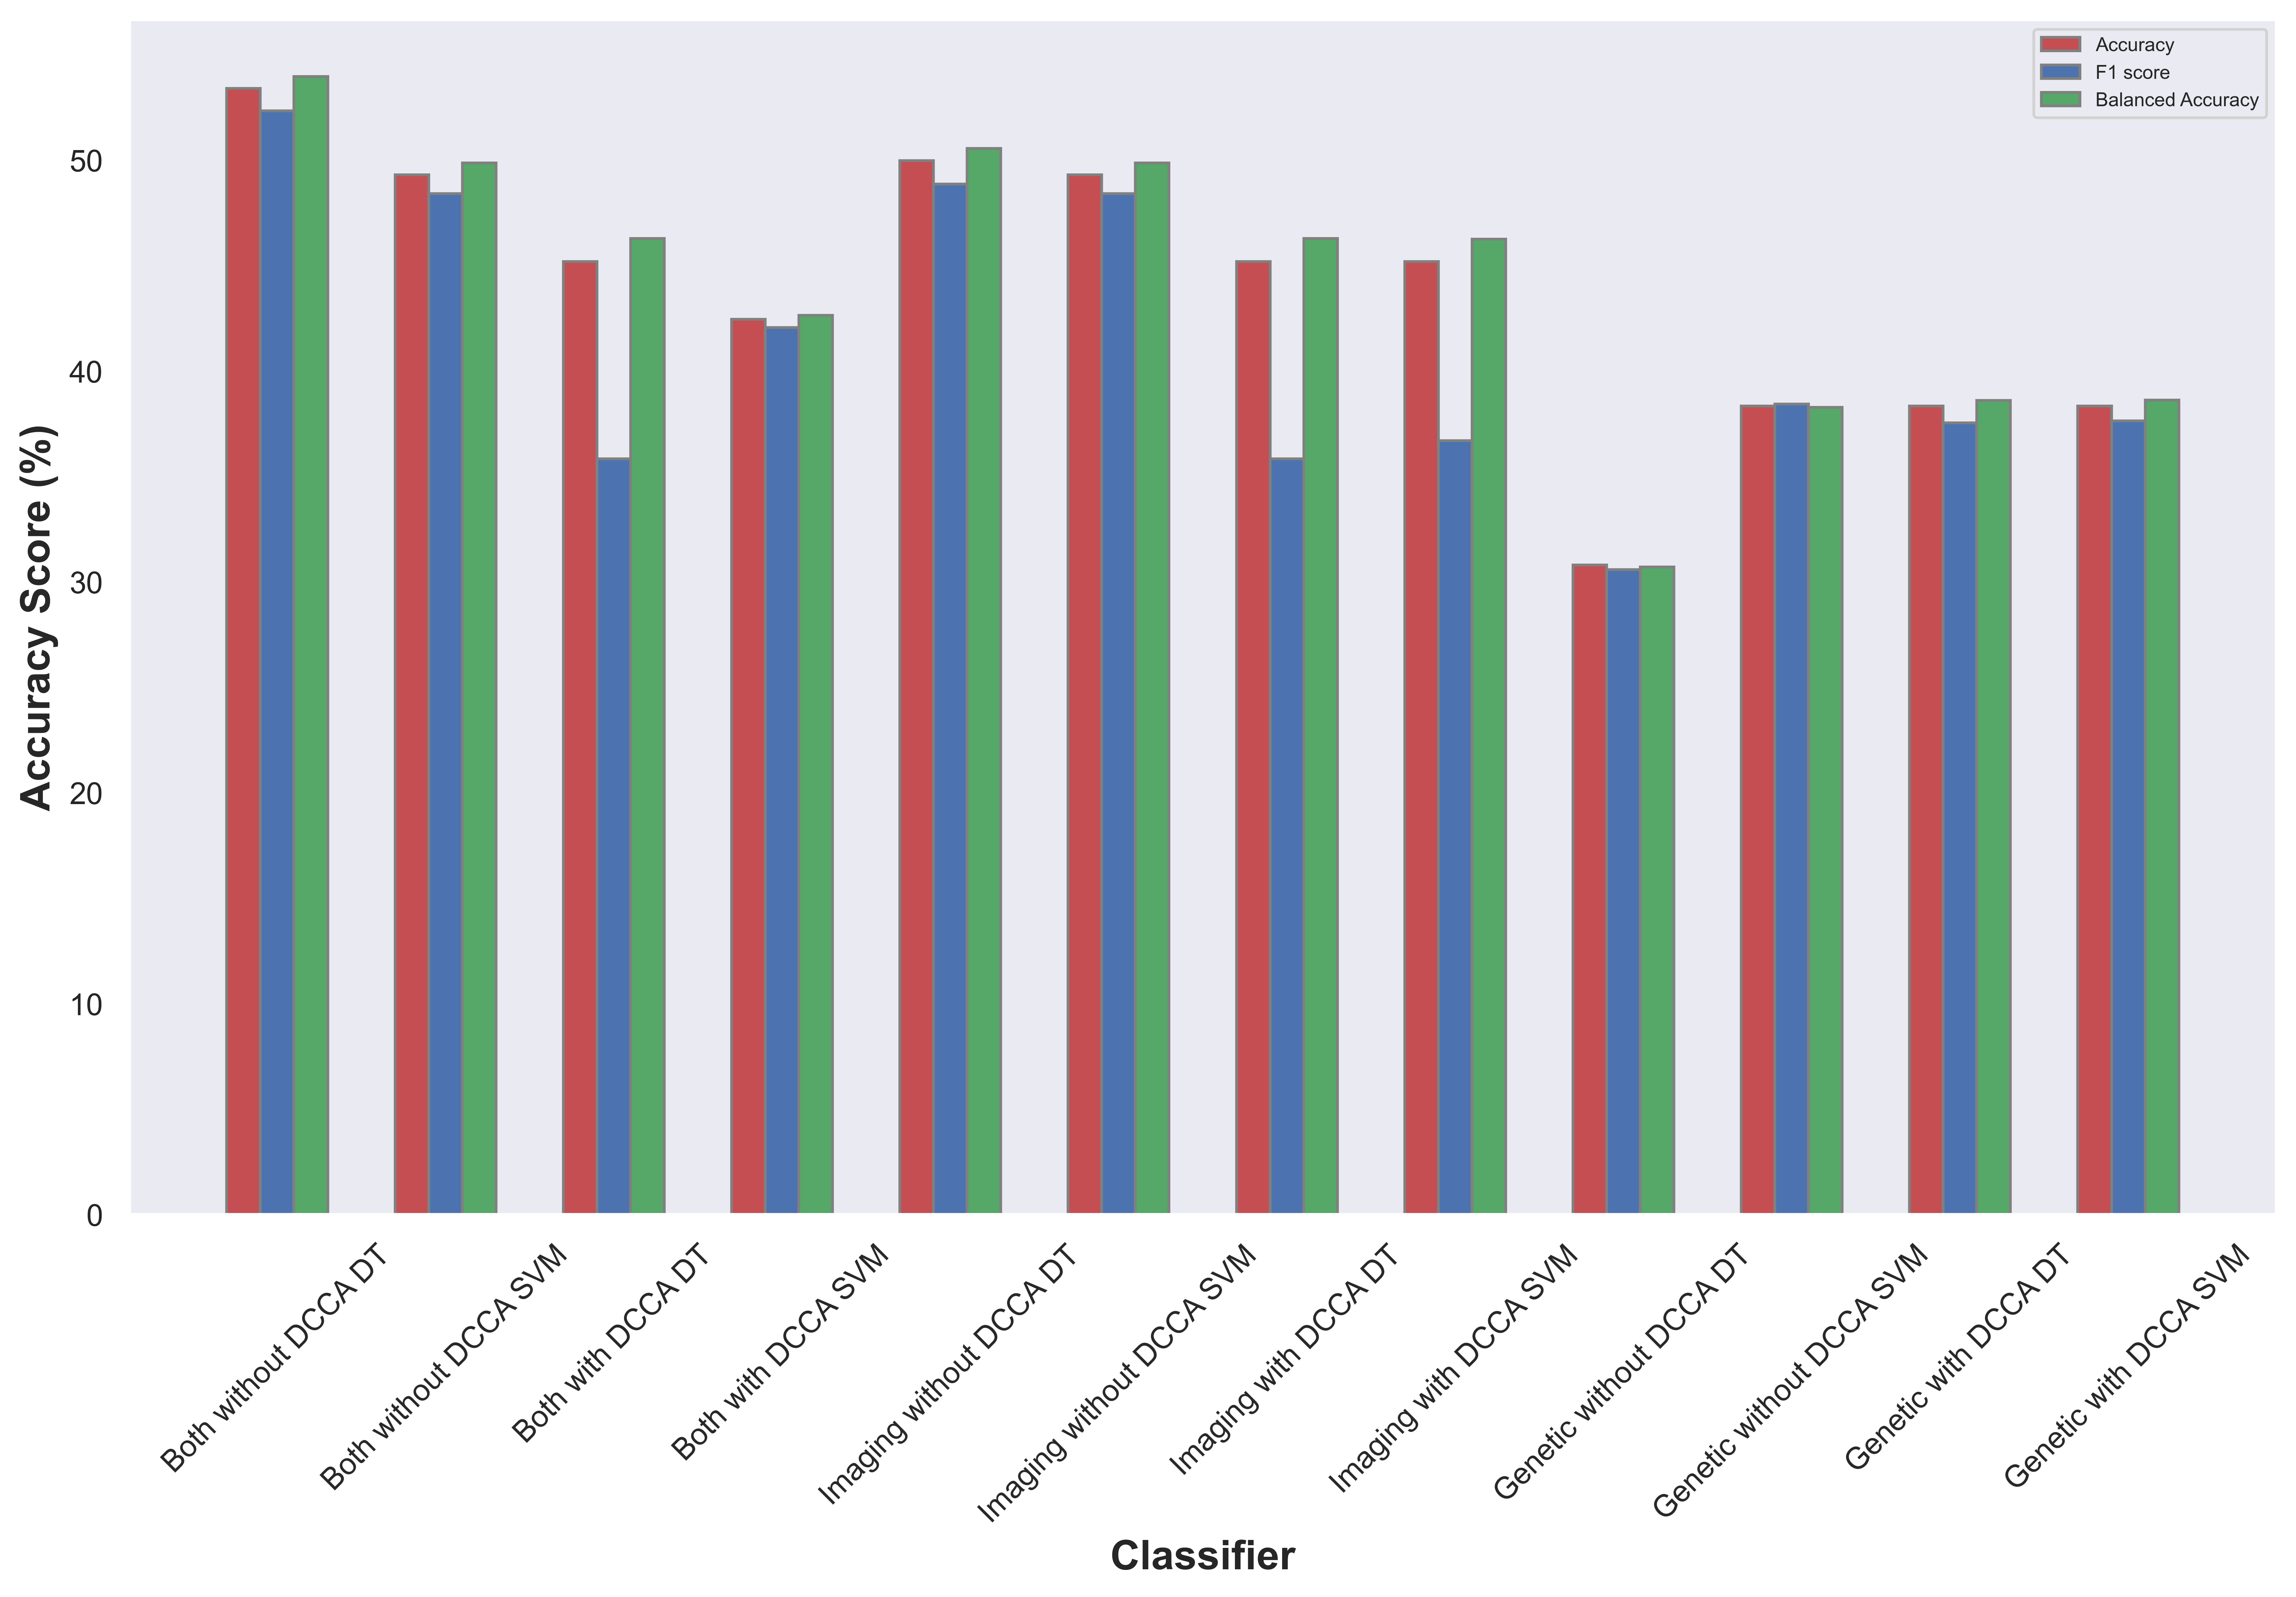
\includegraphics[width=\textwidth]{figures/Results/MCA/AdaBoost_MCA_with.png}
    \caption[\en{MCA AdaBoost Classification metrics with scaling and balancing}]{\en{Classification metric using AdaBoost on the MCA transformed imaging and genetic data.}}
\end{figure}

% \begin{figure}[H]
%     \centering
%     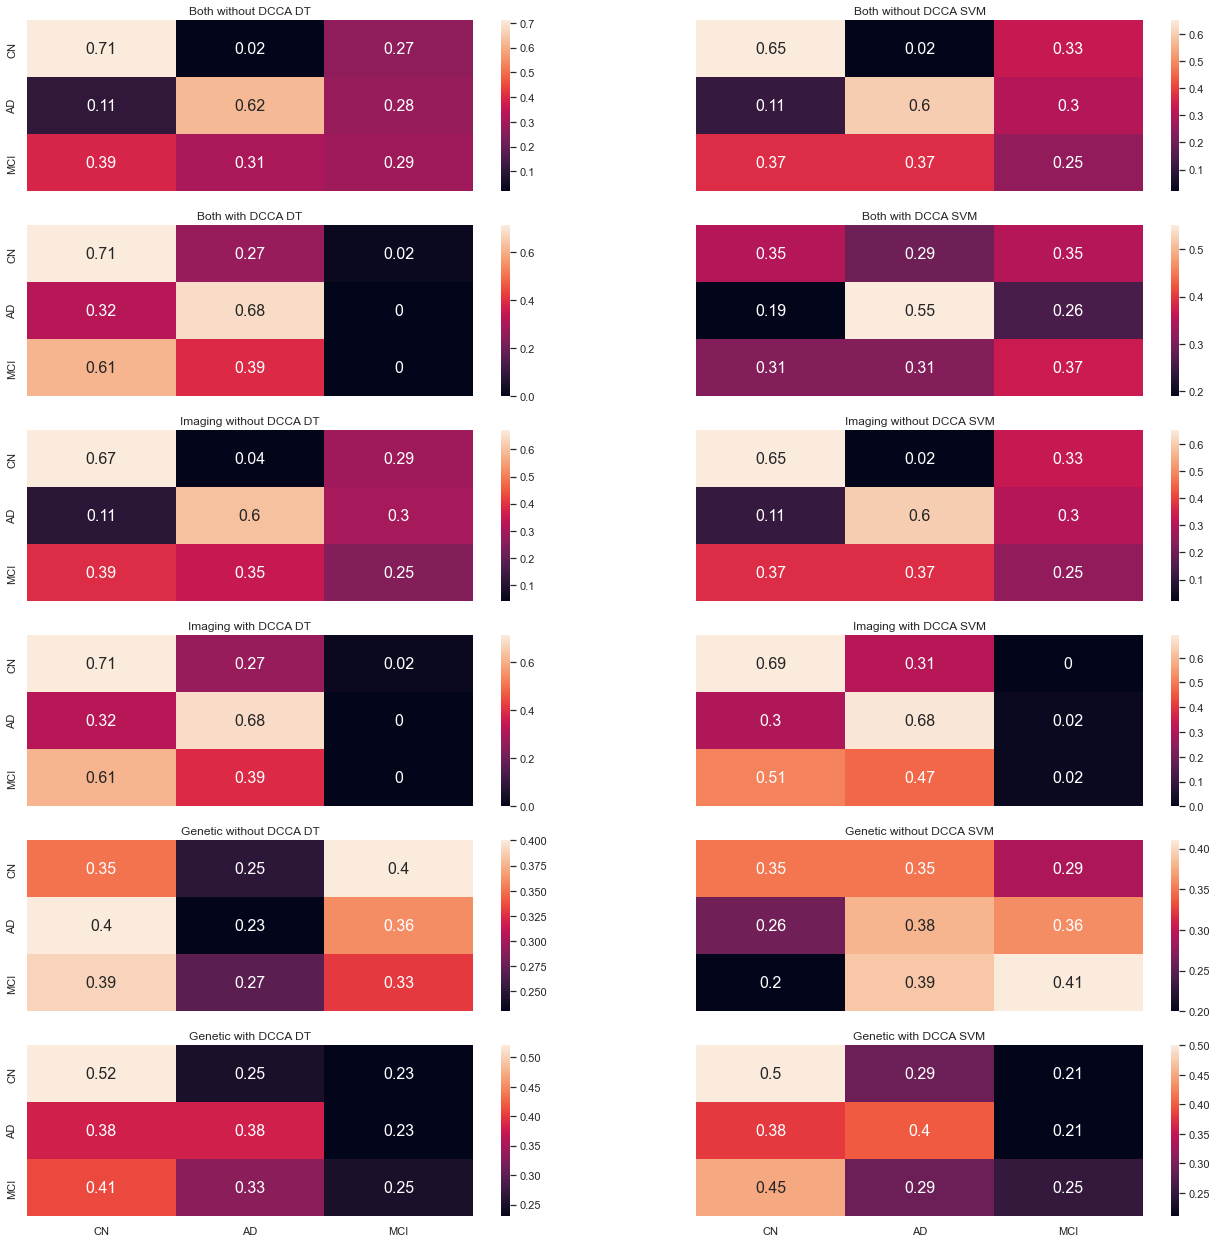
\includegraphics[width=\textwidth]{figures/Results/MCA/AdaBoost_MCA_CM_with.png}
%     \caption[\en{MCA AdaBoost Confusion Matrices with scaling and balancing}]{\en{The Confusion Matrices for each class, with AdaBoost, for the MCA transformed imaging and genetic data.}}
% \end{figure}

The following tables present the complete results for the MCA transformed data, as well as the DCCA transformed data after MCA transformation on the genetic data, for each model, for each metric, for each view, and either with or without scaling and balancing. With green are highlighted the best values for each metric, depending on whether scaling and balancing were applied:

\begin{figure} [H]
    \centering
    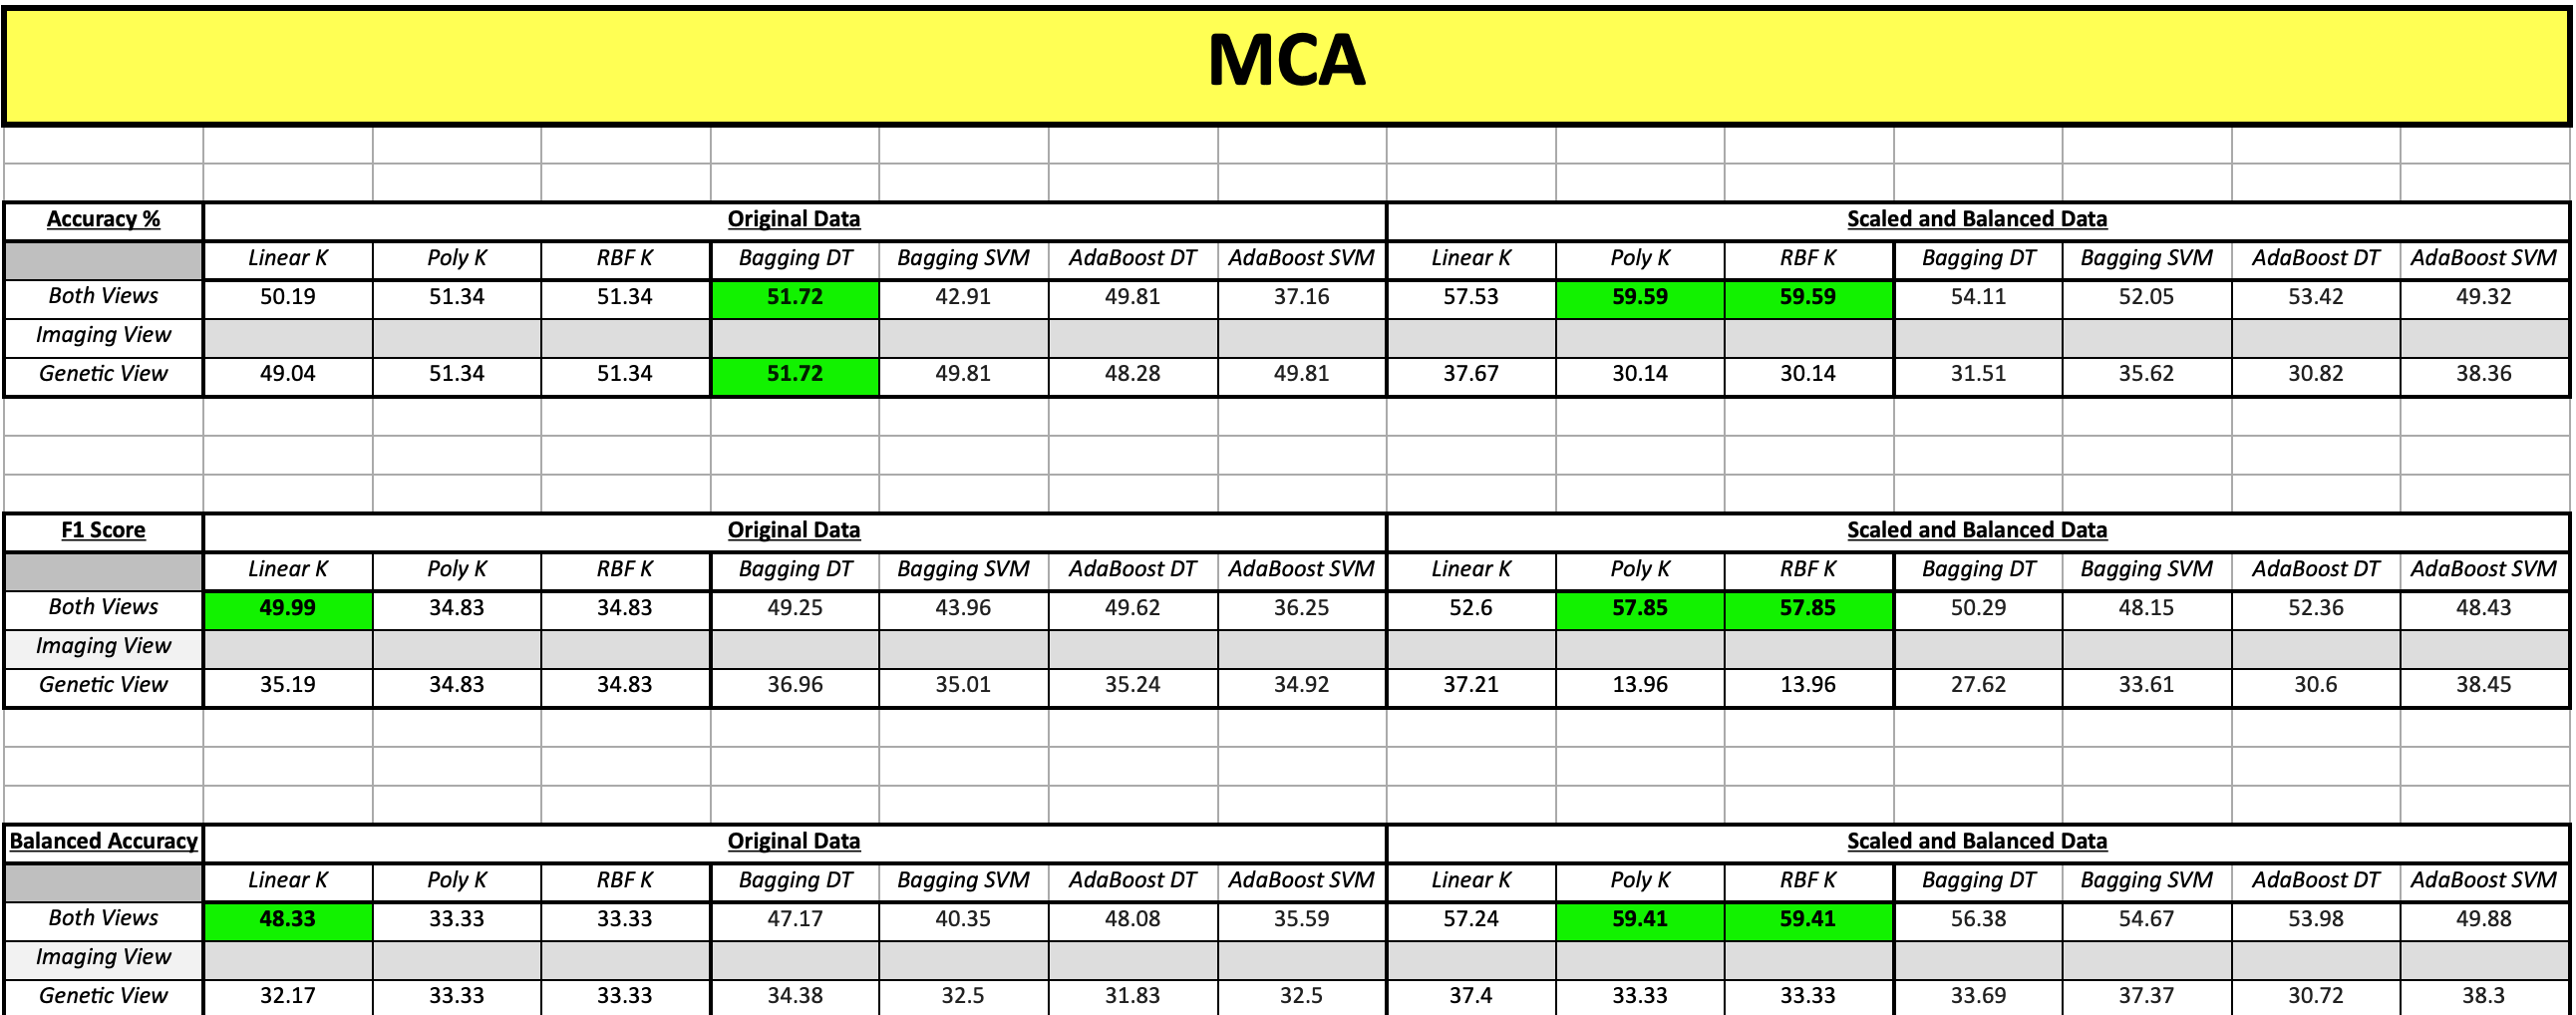
\includegraphics[width=\textwidth]{figures/Results/Analytical_Table_MCA.png}
    \caption[\en{Analytical table of results for MCA data classification}]{\en{For each model and classifier, the metric scores for MCA transformed data classification are presented. Highlighted green are the best performing models, for each metric.}}
    \label{fig: Summary Table for classification scores for MCA transformed data}
\end{figure}

\begin{figure} [H]
    \centering
    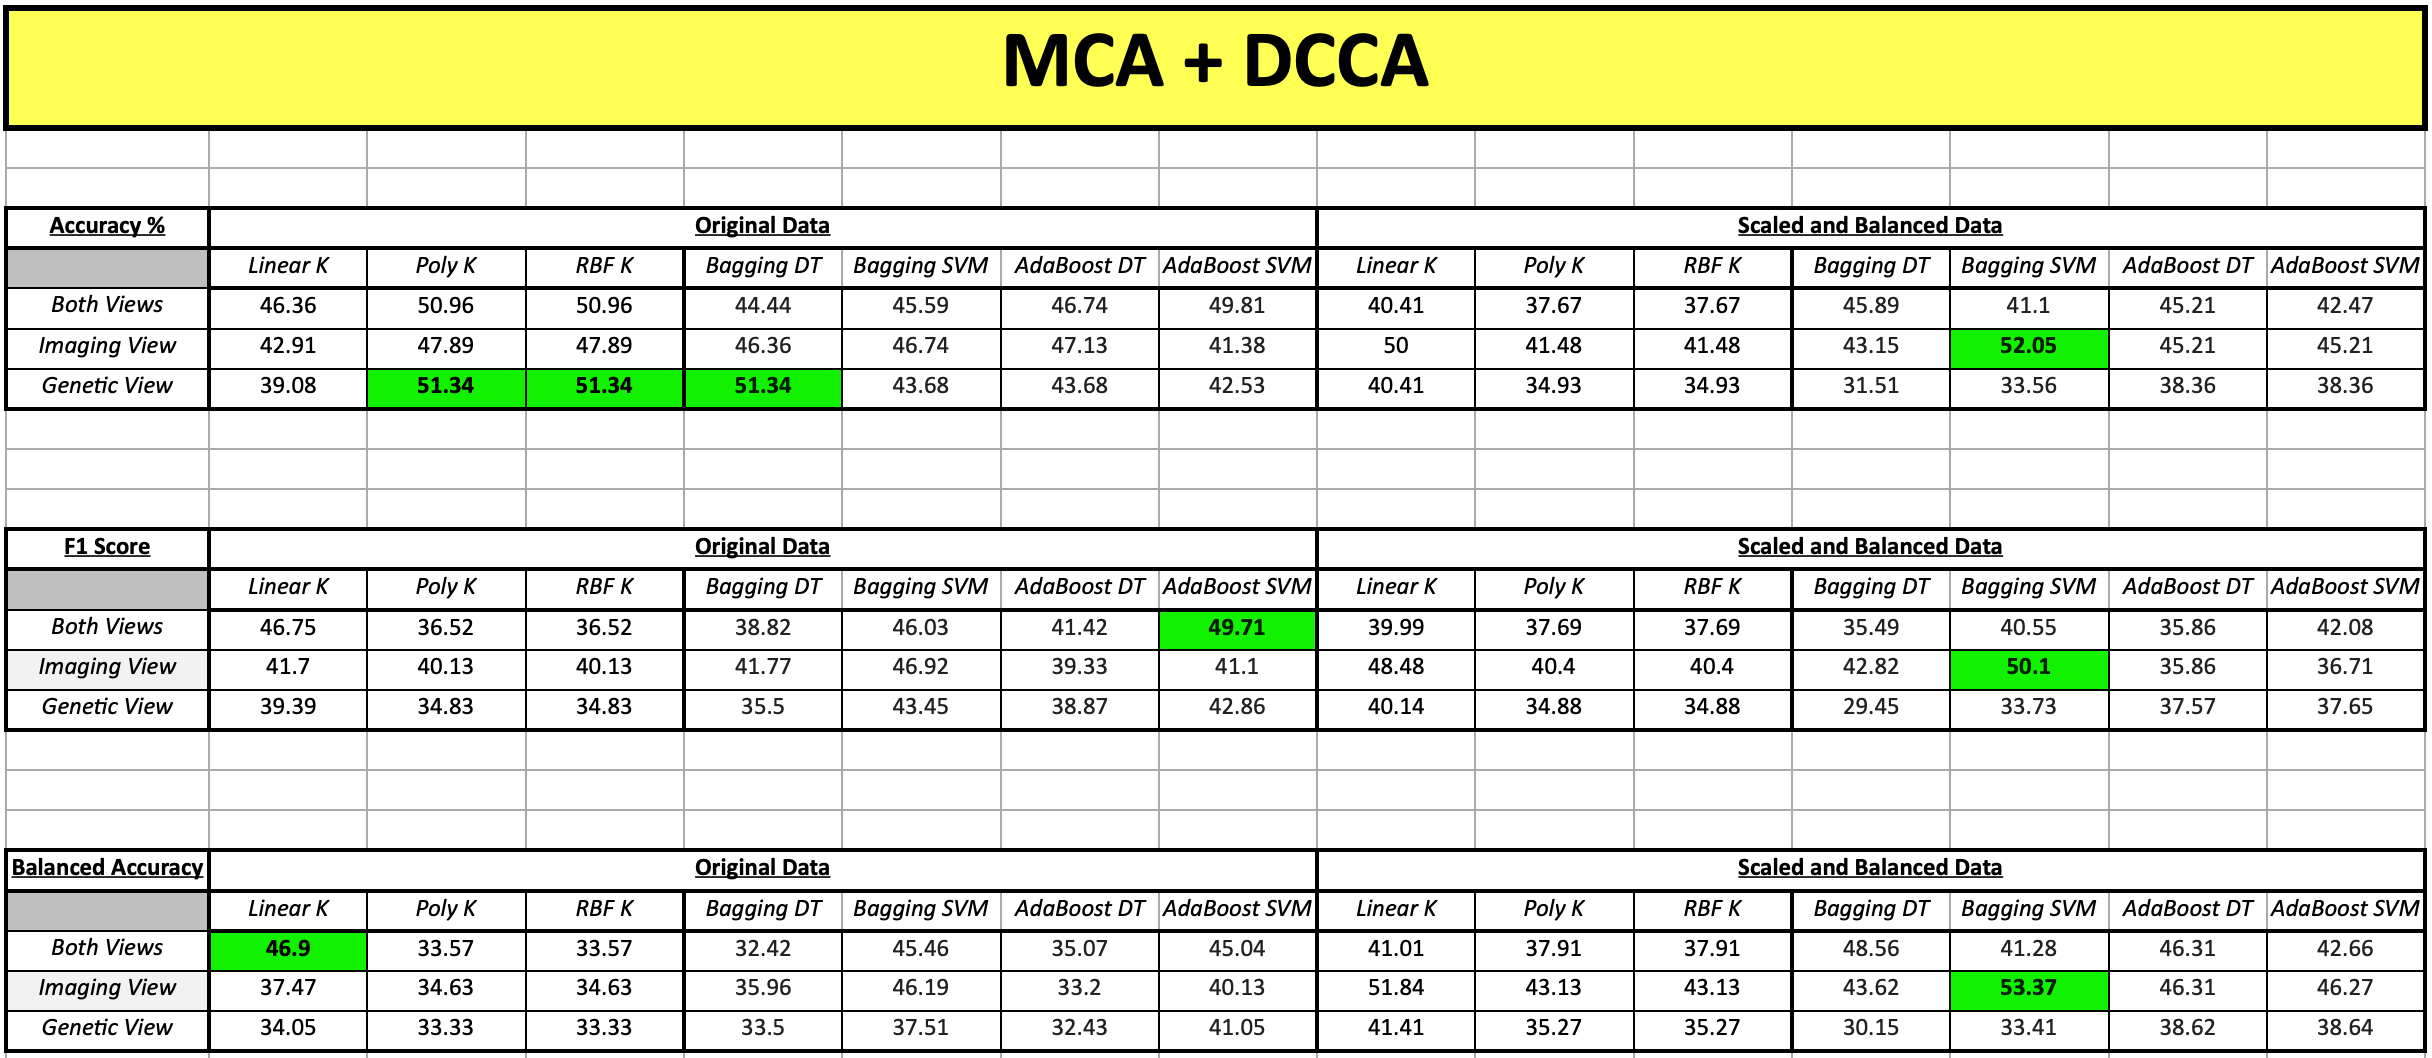
\includegraphics[width=\textwidth]{figures/Results/Analytical_Table_MCA_DCCA.png}
    \caption[\en{Analytical table of results for MCA-DCCA transformed data classification}]{\en{For each model and classifier, the metric scores for MCA - DCCA transformed data classification are presented. Highlighted green are the best performing models, for each metric.}}
    \label{fig: Summary Table for classification scores for MCA - DCCA transformed data}
\end{figure}

}